\chapter{Další kroky v návrhu}\label{chap:kroky}
V předchozí kapitole jsem vytvořil základní model rotorového listu. Tento list však má spoustu nevyjasněných prvků, které Gluertova teorie nepokrývá. V této kapitole bych se na ně chtěl zaměřit a probrat je.

\section{Oblast kolem středu, startovatelnost}
Ve většině konstrukcí amatérských větrných turbín si lze všimnout, že autoři záměrně vypouští část listu blízko osy otáčení. Např. v knize \cite{Crome:Technika} autoři vypouští polovinu poloměru. Obdobně i různí autoři uvedení v knize \cite{Hallenga:Elektrarna} vypouští oblast kolem středu.

Tato oblast je vypouštěna nejen díky nízkému výkonu (viz. graf \ref{graf.vykon}), ale také díky dlouhé tětivě, tudíž i větší spotřebě materiálu. Navíc profil v tomto místě omezuje nosnou konstrukci.
\begin{figure}[H]
	\centering
	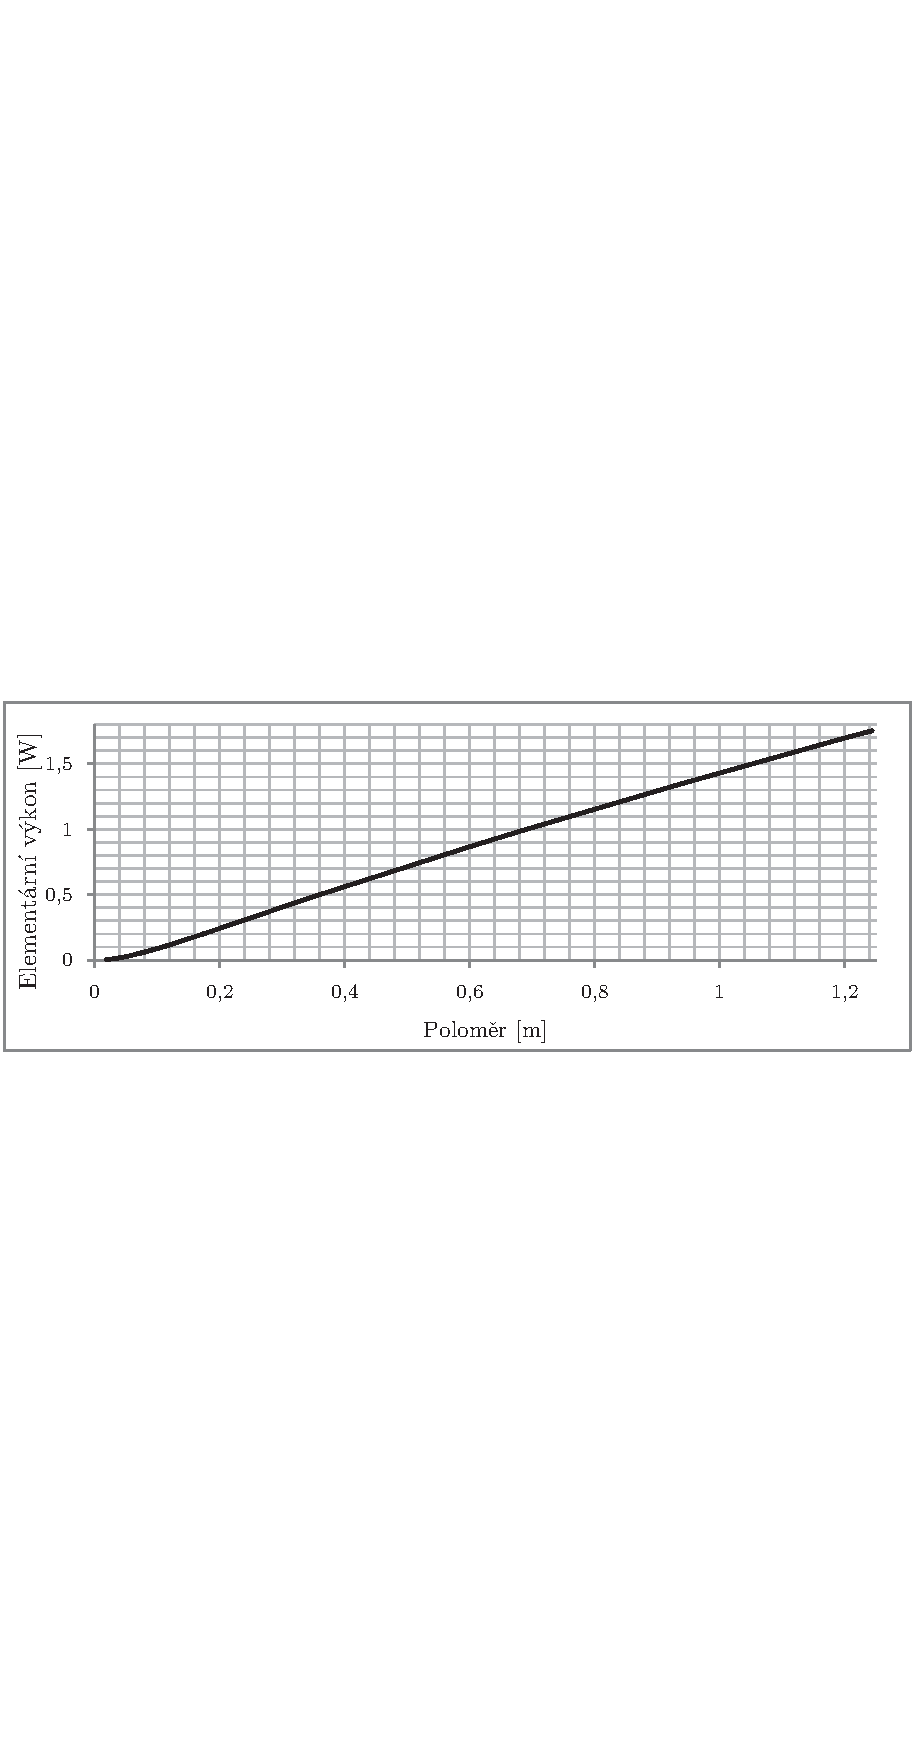
\includegraphics[]{obrazky/grafy/vykonp}
	\caption{Výkon jednotlivých elementů na poloměru $r$}
	\label{graf.vykon}
\end{figure}
V mém návrhu tuto oblast nevypouštím, jelikož se nejvíce podílí na startovatelnosti, která je v turbulentním prostředí důležitá. Na první pohled tato informace vypadá jako nesmysl – síla zde působí na krátké páce a vyvolává malý krouticí moment. Podstata startovatelnosti spočívá jinde.

Veškeré teorie uvažují konstantní rychloběžnost, která však při rozběhu rotoru nenastává. Rotor má menší (resp. nulové) otáčky díky čemuž se mění i směr relativní rychlosti proudu vzduchu a profil není ofukován pod optimálním úhlem, tudíž na něm nevzniká tak velký vztlak (naopak narůstá odpor). Tato odchylka se se vzrůstající rychloběžností zvětšuje. A právě v~oblasti blízko osy rotace je rychloběžnost jednotlivých elementů listu velmi malá, díky čemuž je i~odchylka od ideálního úhlu náběhu malá. K lepší startovatelnosti také významně pomáhá profil, který má charakteristiku podobnou grafu \ref{graf.jemnost1}. Profil je \uv{tolerantnější} k úhlu náběhu a podává dobré výsledky i při nekonstantní rychloběžnosti.

Jelikož má tato oblast listu relativně malou obvodovou rychlost $u$, nezpůsobí zde změna tvaru profilu příliš velký rozdíl v~jeho vlastnostech. Proto je výhodné v této oblasti zvýšit tloušťku profilu a získat více prostoru pro nosnou konstrukci. Tuto změnu tloušťky jsem však do mého CAD modelu zatím nezanesl – ještě nejsou přesně známy technické detaily ohledně realizace rotorových listů.

\section{Zakončení listů}
Gleurtova teorie, stejně jako i ostatní, přepokládají, že rotor má nekonečný počet nekonečně tenkých lopatek. V praxi se však ničemu takovému nelze přiblížit.

Malý počet lopatek se projevuje aerodynamickými ztrátami. Příčinu těchto ztrát lze vysvětlit rozdílným tlakem na tlakové a podtlakové straně aerodynamického profilu. Díky tomuto rozdílu se vzduch na konci listu \uv{přelévá} z tlakové strany na podtlakovou ve snaze tento rozdíl vyrovnat. Tím uděluje proudu vzduchu rotační složku a na konci lopatky tak vzniká tzv. indukovaný vír. Tento vír snižuje vztlakovou sílu na konci listu a je také jednou z příčin hlučnosti větrných turbín.

Nenašel jsem žádnou literaturu, která by se problémem indukovaných vírů u větrných turbín zabývala. Literaturu zabývající se snížením ztrát u křídel letadel lze najít, avšak není příliš podrobná. Většinou jsou v ní indukované víry pouze zmíněny a možnosti, jak je omezit, jsou uvedeny pouhým výčtem. Nenašel jsem nikde popis, jak má např. vypadat winglet, aby měl správnou funkci.

Rozhodl jsem se proto jít experimentální cestou. Jelikož jsou však praktické pokusy časově, materiálně a technicky náročné, rozhodl jsem se využít CFD simulace.

Nesnažil jsem se o odvození teorie, pouze jsem chtěl zjistit, jak lze list rotoru ukončit, aby se snížily indukované ztráty (a potenciálně i hlučnost). Připravil jsem si šest různých zakončení rotorového listu, která jsem následně otestoval v simulaci. Inspiraci pro tato zakončení jsem čerpal z různých zdrojů. Od křídel dopravních letadel, přes fotografie větrných elektráren až po RC modely.

Jako simulační software jsem použil studentskou verzi Autodesk Simulation Multiphysics. Původně jsem plánoval použít open-source projekt OpenFOAM\footnote{http://www.openfoam.com/}. Ten je na rozdíl od Autodesk Simulation komplexnější, více přizpůsobitelný, avšak jedná se spíše o C++ framework, než program pro koncového uživatele. OpenFOAM nemá žádné GUI, veškerý vstup se do něj zadává pomocí zdrojových kódů. Naučit se tento program používat je na dlouhou dobu. Proto jsem se rozhodl, že použiji uživatelky přívětivější Autodesk Simulation.

Jelikož jsou CFD simulace relativně početně náročné, neprováděl jsem je na celém listu. Simulace jsem prováděl na posledních 25 centimetrech listu. Zde se úhel náběhu již příliš nemění, a je tedy proto možné tento úsek ofukovat pod stejným úhlem bez velké změny na vlastnostech. To opět zjednodušuje simulaci.

Simulaci jsem prováděl v bounding-boxu o rozměrech 100 $\times$ 80 $\times$ 40 cm (délka za listem, prostor ve směru listu, prostor pod a nad listem). Tato oblast je relativně malá. Díky tomu výpočet neprobíhal příliš dlouho (zhruba hodinu). Ovšem jak ukázaly výsledky, tato oblast byla pro některá zakončení malá a výsledky byly ovlivněny stěnami bounding-boxu. Avšak pro mé účely, kdy nepotřebuji přesné hodnoty, pouze porovnávám několik případů, je tato nepřesnost opomenutelná.

Simulace jsem prováděl pro rychlost větru 5~$m\cdot s^{-1}$, konec listu jsem tedy ofukoval proudem vzduchu s rychlostí 25~$m\cdot s^{-1}$ (zanedbal jsem vektorový součet rychlostí). Byla použita simulace typu \uv{Unsteady fluid flow}, která je manuálem pro aerodynamické simulace doporučována. Simuloval jsem dobu 5 sekund, rozdělenou na 200 snímků. Pro počet iterací mezí jsem ponechal standardní hodnotu 15. Proud vzduchu byl spuštěn bez vzestupné rampy (tzn. od začátku simulace měl zadanou rychlost, rychlost byla po celou dobu konstantní).

První simulaci jsem provedl na prostém ukončení listu beze změn, abych měl s čím výsledky porovnávat. Na této simulaci jsem také zkoušel, jak porovnávat výsledky. Ukázalo se, že na znázornění rychlosti (obrázky \ref{sim:2} a \ref{sim:3}), ani grafech rychlosti jednotlivých bodů není nic poznat. Lehce průkazné bylo znázornění rychlosti ve směru osy X při pohledu zezadu na list (pohled proti směru proudícího vzduchu, obrázek \ref{sim:1}), kde lze vidět, jak se proud vzduchu pohybuje nad listem  na opačnou stranu než proud vzduchu pod listem. Avšak z tohoto znázornění lze pouze vyčíst existenci víru. Nelze určit jeho tvar, rychlost, ani jakou oblast listu ovlivňuje.

O víru toho nejvíce vypovídají proudnice. Proudnice jsou křivky, které mají v každém svém bodě směr rychlosti proudu vzduchu. Při pohledu zezadu listu (proti směru proudu vzduchu) je na nich jasně vidět vznikající vír, jeho velikost, pozice a rychlost. Z tohoto pohledu si lze vytvořit celkem jasnou představu o vznikajícím víru. Mírné doplnění poskytne i pohled shora, kde je vidět jak proudnice vybočují z rovnoběžného směru.

\begin{figure}[H]
	\centering
	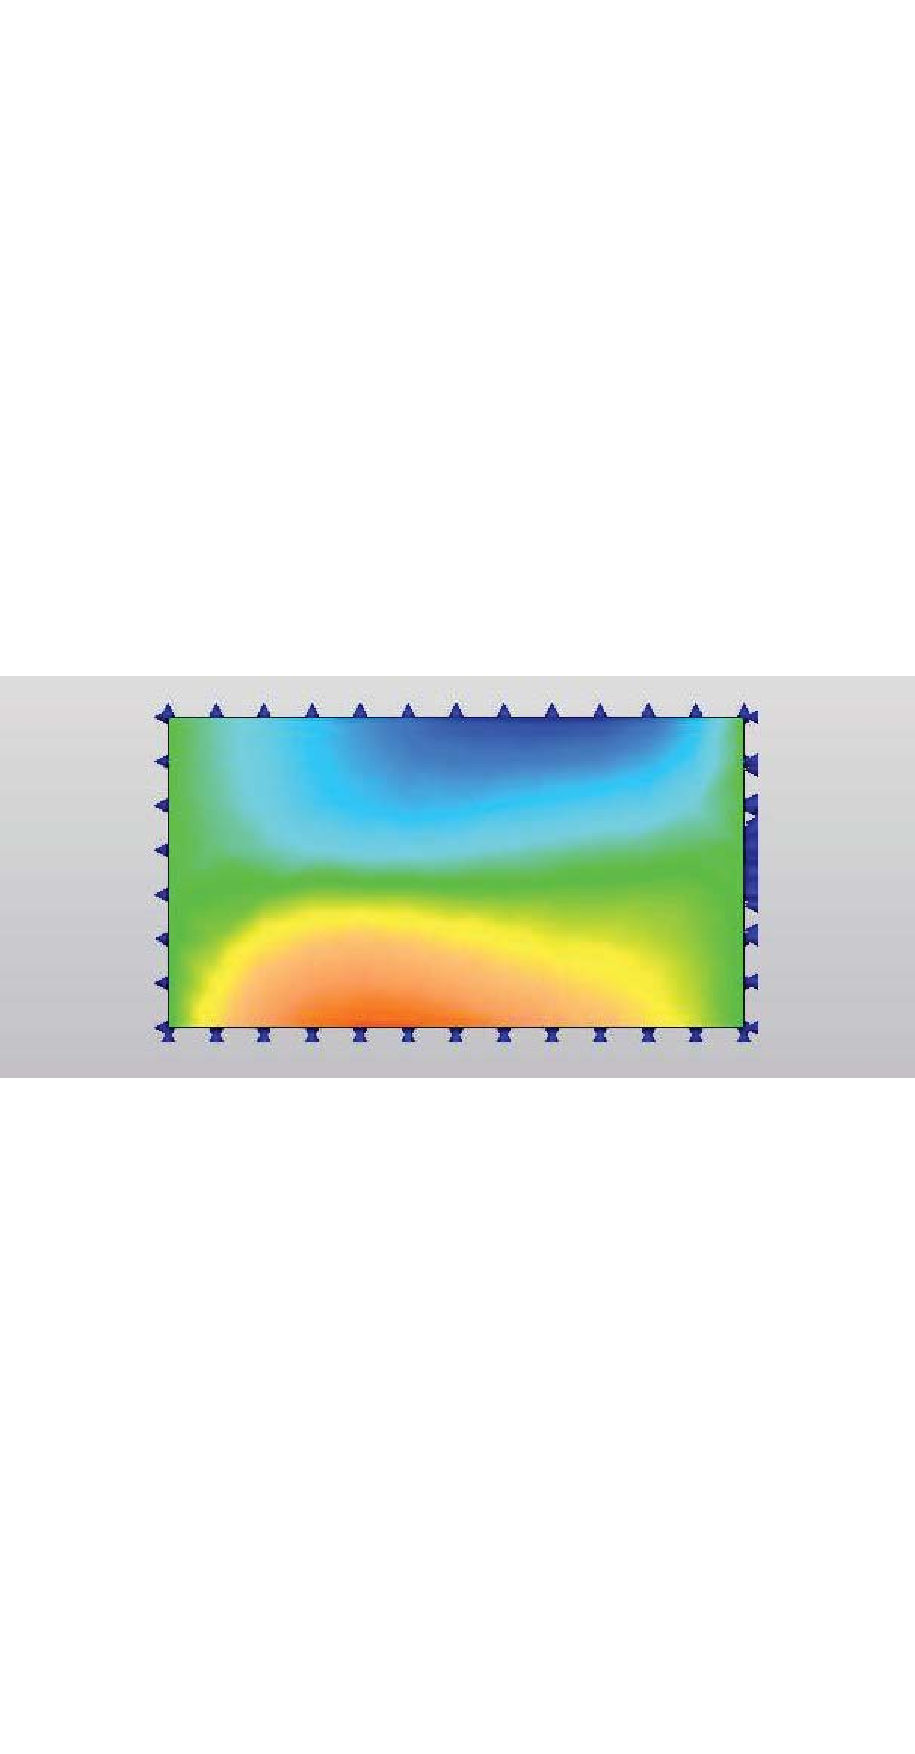
\includegraphics[]{obrazky/simulace/simulace1p}
	\caption{Zde je vidět projev víru – červená barva znázorňuje pohyb vzduchu doleva, modrá doprava. Zelená barva značí nulovou rychlost.}
	\label{sim:1}
\end{figure}
\begin{figure}[H]
		\centering
		\subfigure[Velikosti rychlosti]{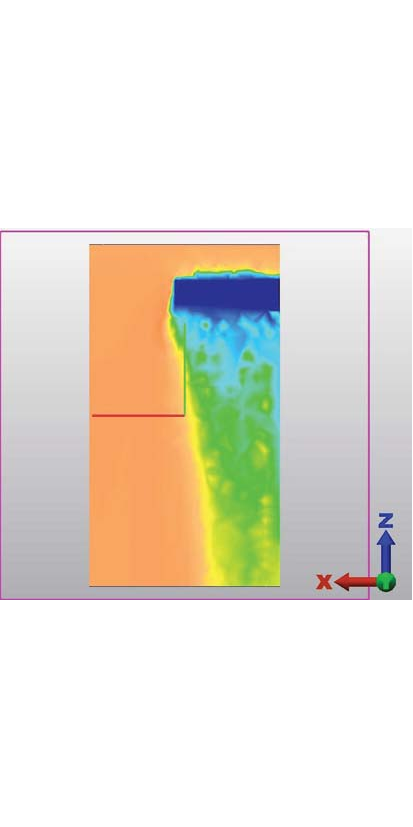
\includegraphics[]{obrazky/simulace/simulace2p}\label{sim:2}}~
		\subfigure[Velikosti rychlosti ve směru osy X]{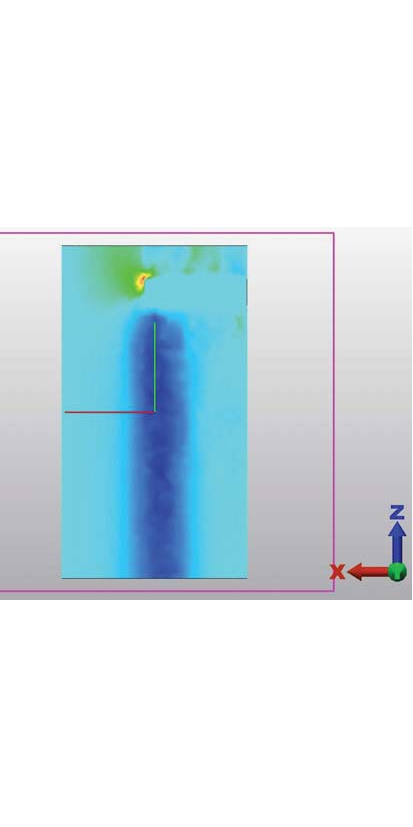
\includegraphics[]{obrazky/simulace/simulace3p}\label{sim:3}}
		\caption{Neprůkazné znázornění výsledků}
	\end{figure}


Na obrázku \ref{sim:4} jsou zobrazeny výsledky simulace listu bez jakéhokoliv zakončení. Z proudnic na tomto obrázku lze jasně vypozorovat vír, který vzniká za listem. Jelikož se proudnice při pohledu zezadu jeví dlouhé, pohybuje se vír velkou úhlovou rychlostí.

Při podrobnějším zkoumání jsem si všiml, že víru jsou dva – velký na tlakové straně a menší na podtlakové. Velký vír také zasahuje více do oblasti samotného listu, naopak malý vír se nachází až za okrajem listu. Průměr velkého víru se pohybuje mezi 20–25~cm. Malý vír má průměr menší než 10~cm. Na proudnicích lze také vidět jasný tok vzduchu mezi tlakovou a~podtlakovou stanou.

Při pohledu shora si můžeme všimnout, že vír nejznatelněji ovlivňuje posledních 15~cm listu. Na opačnou stranu je koncem listu ovlivněn i vzduch 6~cm vzdálený od konce listu.

\begin{figure}[H]
	\centering
	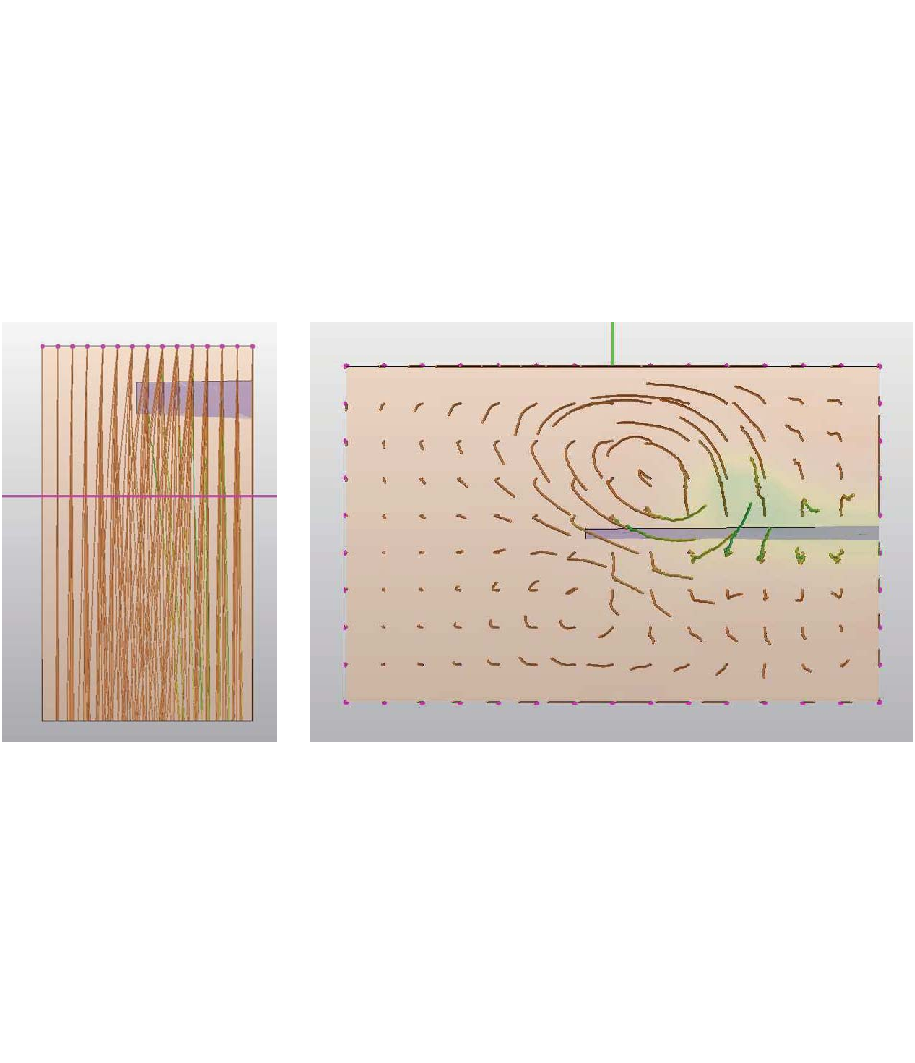
\includegraphics[]{obrazky/simulace/simulace4p}
	\caption{Proudnice listu bez zakončení. Na obrázku vpravo je jasně patrný vír za listem. Na obrázku vlevo lze vidět, jak na konci listu přestávají být proudnice rovnoběžné.}
	\label{sim:4}
\end{figure}

\subsection{Zakončení odsazením}
Autor knihy \cite{Crome:Technika} používá na svých turbínách pro snížení indukovaného odporu přesah na konci listu. Tento přesah, respektive odsazení, má za cíl omezit, popř. i úplně zamezit, toku vzduchu mezi tlakovou a podtlakovou stranou. Toto odsazení má velikost 10 mm, avšak autor má na svém listu mnohem delší tětivu než já. Rozhodl jsem se proto nasimulovat dvě velikosti odsazení – 5 a 10~mm.

Na obrázku \ref{konec:1} si lze prohlédnout model pětimilimetrového odsazení, na kterém byla provedena simulace.
\begin{figure}[H]
	\centering
	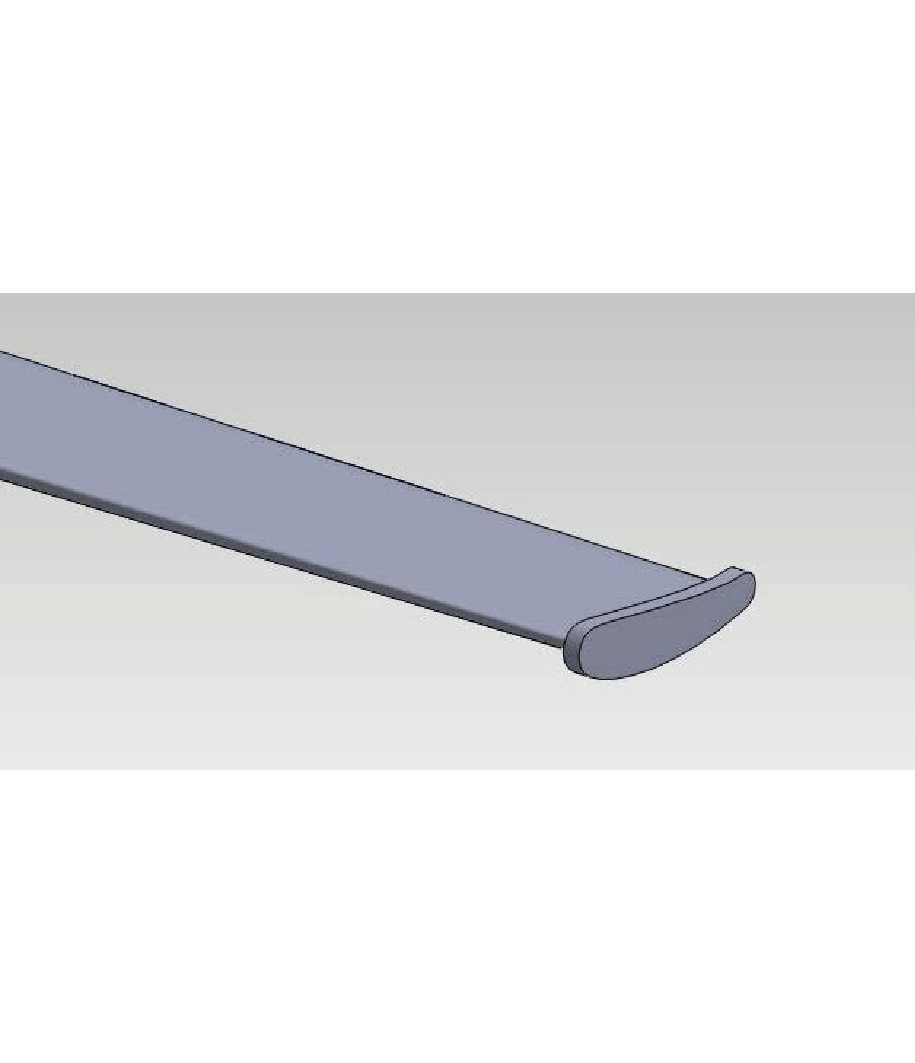
\includegraphics[]{obrazky/simulace/konec1p}
	\caption{Pětimilimetrové odsazení na konci listu}
	\label{konec:1}
\end{figure}

\begin{figure}[H]
	\centering
	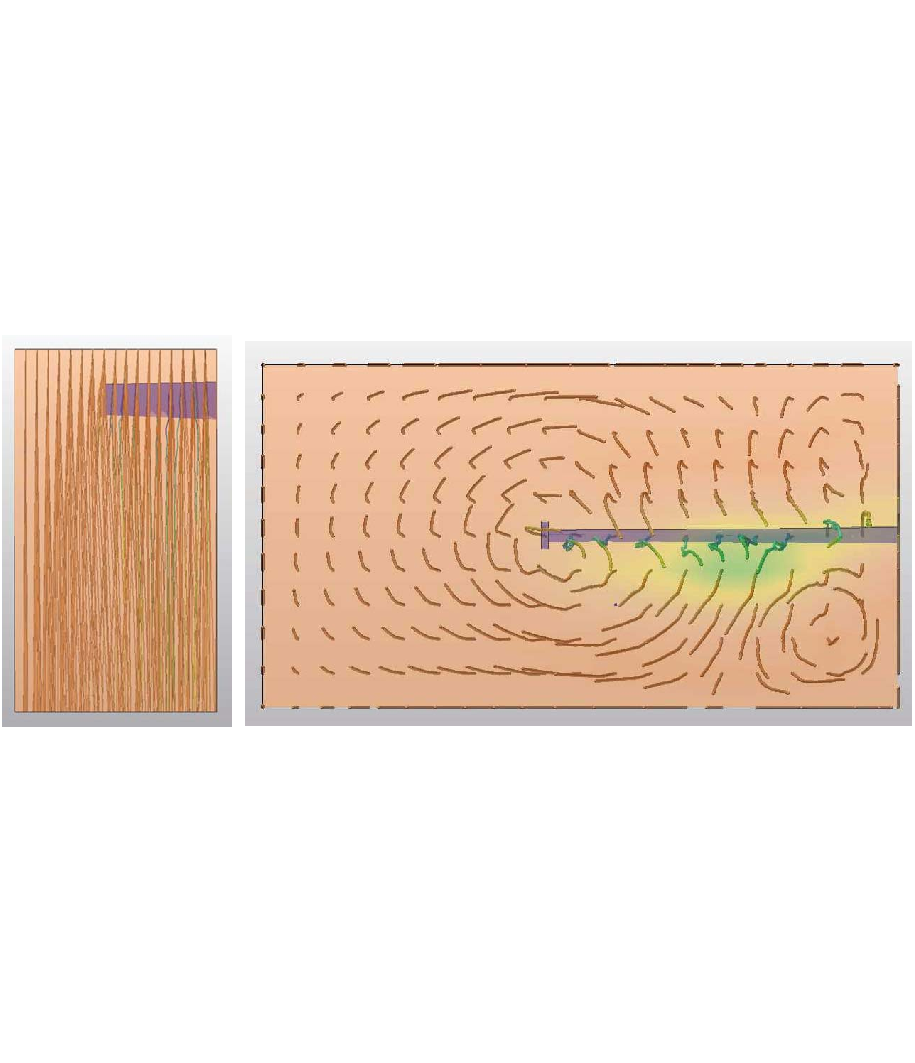
\includegraphics[]{obrazky/simulace/simulace5p}
	\caption{Výsledky pětimilimetrového odsazení na konci listu}
	\label{sim:5}
\end{figure}
Přidání této malé plošky výrazně mění charakter vnikajícího víru, jak je patrné na obrázku \ref{sim:5}. Je vidět, že vzniká pouze jediný vír, není zde přímý tok vzduchu mezi tlakovou a podtlakovou stranou a~úhlová rychlost víru je mnohem menší než v~předchozím případě. Vír se také posunul směrem z~plochy listu a~méně ji ovlivňuje.

Vír, který vzniká v pravém dolním rohu simulace, je způsoben malým simulačním prostorem – proud vzduchu zde ovlivňují stěny.
Při pohledu shora je jasně patrné minimální zakřivení proudnic. Vír tedy velmi rychle zaniká – to je dáno nižší úhlovou rychlostí.

Jinak však vypadá situace pro desetimilimetrové odsazení (obrázek \ref{sim:6}). Zde vzniká v místě zakončení proud s velkou úhlovou rychlostí obklopen druhým proudem s nízkou rychlostí. Při trojrozměrném zobrazení je vidět, že tento pomalý vír velmi rychle zaniká, avšak vnitřní vír pokračuje dále.

\begin{figure}[H]
	\centering
	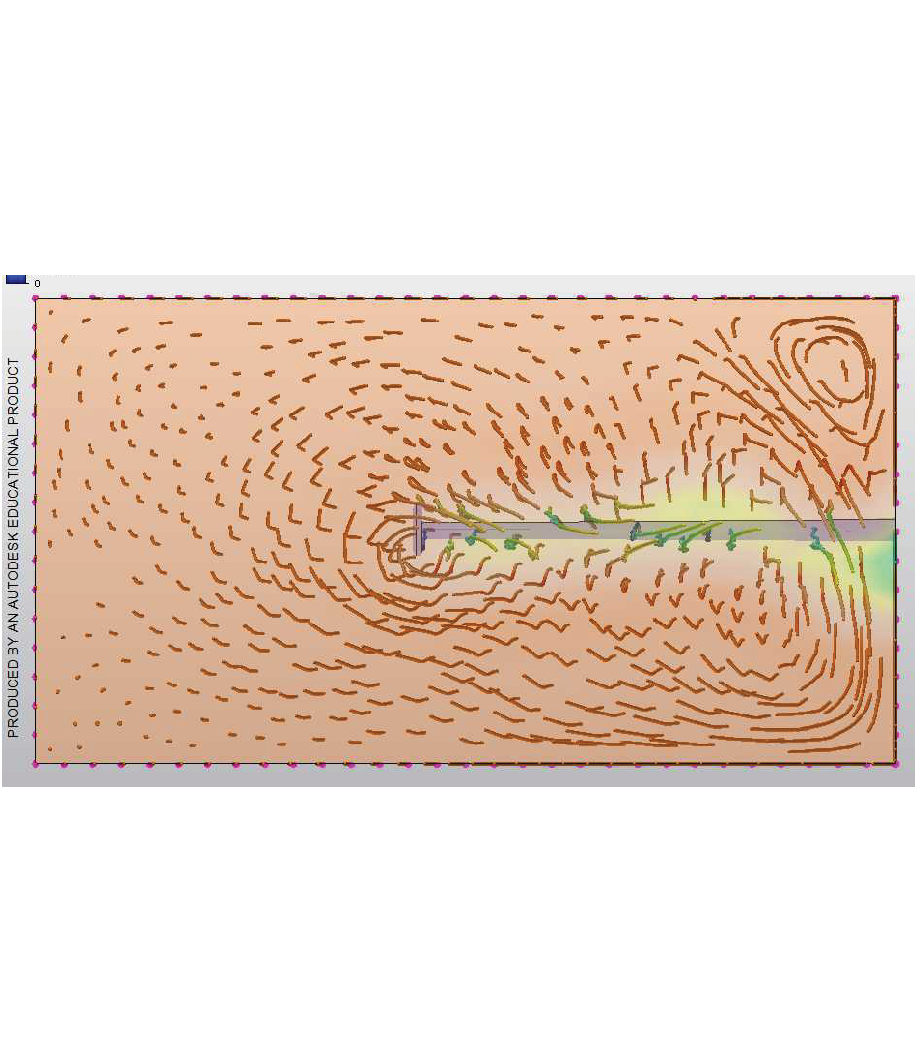
\includegraphics[]{obrazky/simulace/simulace6p}
	\caption{Výsledky desetimilimetrového odsazení na konci listu}
	\label{sim:6}
\end{figure}

Můj původní předpoklad, že délku velikost odsazení je nutno přizpůsobit délce tětivy, se ukázal jako správný. Simulace ukazuje, že pětimilimetrové odsazení pravděpodobně funguje. Díky víru s malou úhlovou rychlostí vznikají nízké ztráty a díky absenci oblasti, kde přetéká vzduch z~tlakové strany na podtlakovou, omezuje vznik hluku. Navíc výroba odsazení není technicky náročná.

\subsection{Zakončení wingletem}
Winglet je zahnutý konec křídla u letadla. Funguje na podobném principu jako odsazení – brání vzduchu proti přetékání mezi stranami aerodynamického profilu. Tím, že je však tvořen aerodynamickým profilem, vyvolává dodatečný vztlak. Poprvé byl v~praxi použit na letadle NASA \cite{winglet}.

Při použití wingletu jsem vycházel z toho, že list rotoru je jednak podobný křídlu letadla, ale také z toho, že na některých velkých větrných elektrárnách je použit. Lze ho najít také na některých typech lodních šroubů.

Bohužel jsem nenašel žádnou literaturu, která by se přímo návrhem wingletu dostatečně zabývala. Jeho tvar jsem sestavil na základě fotografií některých křídel letadel a velkých větrných elektráren. Avšak takovéto sestavení je značně nedostatečné.

Sestavil jsem 2 modely (obrázek~\ref{konec:2}) - jeden winglet zahnutý o $85\,^{\circ}$ a druhý o $65\,^{\circ}$. Winglet jsem nasměroval na podtlakovou stranu jako u křídla letadla. Winglet má stejný profil jako celý list. Délka tětivy se lineárně zmenšuje až na polovinu původní délky.

\begin{figure}[H]
	\centering
	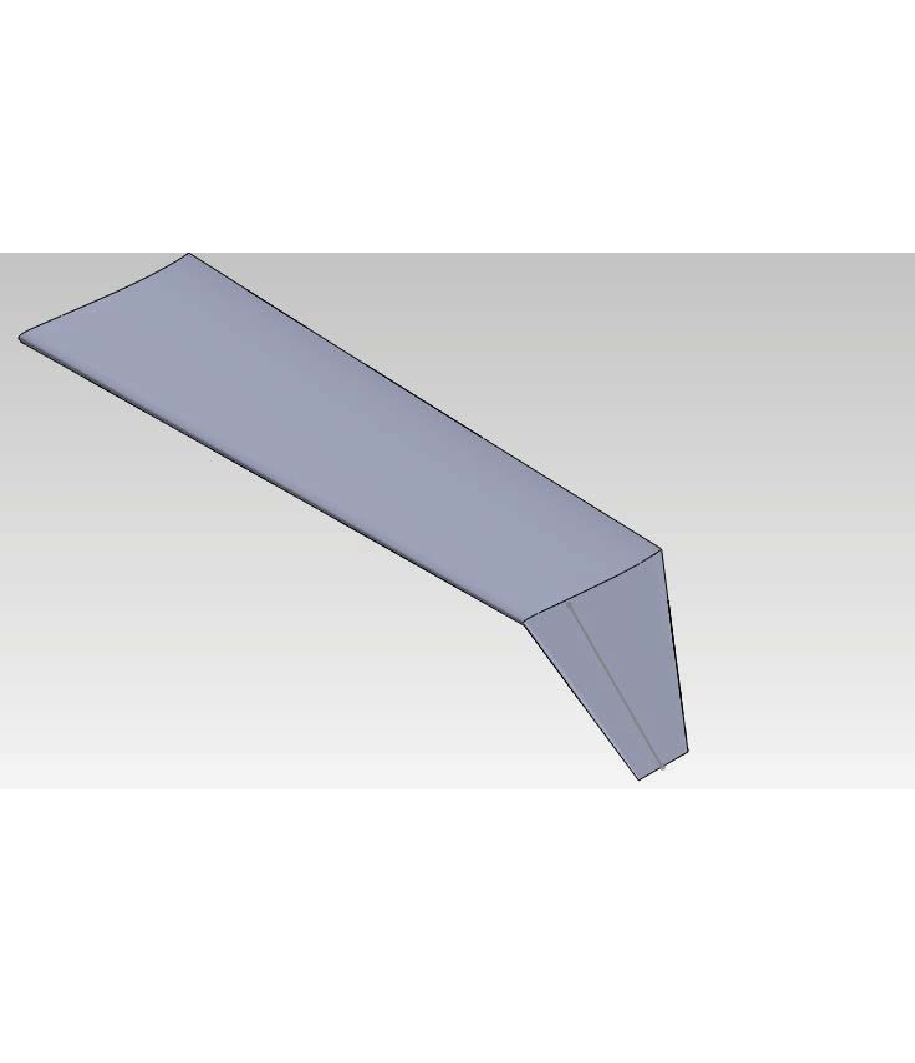
\includegraphics[]{obrazky/simulace/konec2p}
	\caption{Model wingletu}
	\label{konec:2}
\end{figure}
Od takto sestaveného modelu jsem nečekal žádné zázračné výsledky. Avšak výsledky mě překvapily – díky wingletu se odklonem $65\,^{\circ}$ vznikal za rotorem vír velkého průměru s velkou úhlovou rychlostí (obrázek \ref{sim:7}). Winglet dokonce silně ovlivňoval proud kolem celé délky simulované části profilu.

Winglet s odklonem $85\,^{\circ}$ vykazoval mnohem lepší výsledky (obrázek \ref{sim:8}) – vznikal téměř neznatelný vír s malou oblastí rychlého proudění vzduchu.

\begin{figure}[H]
	\centering
	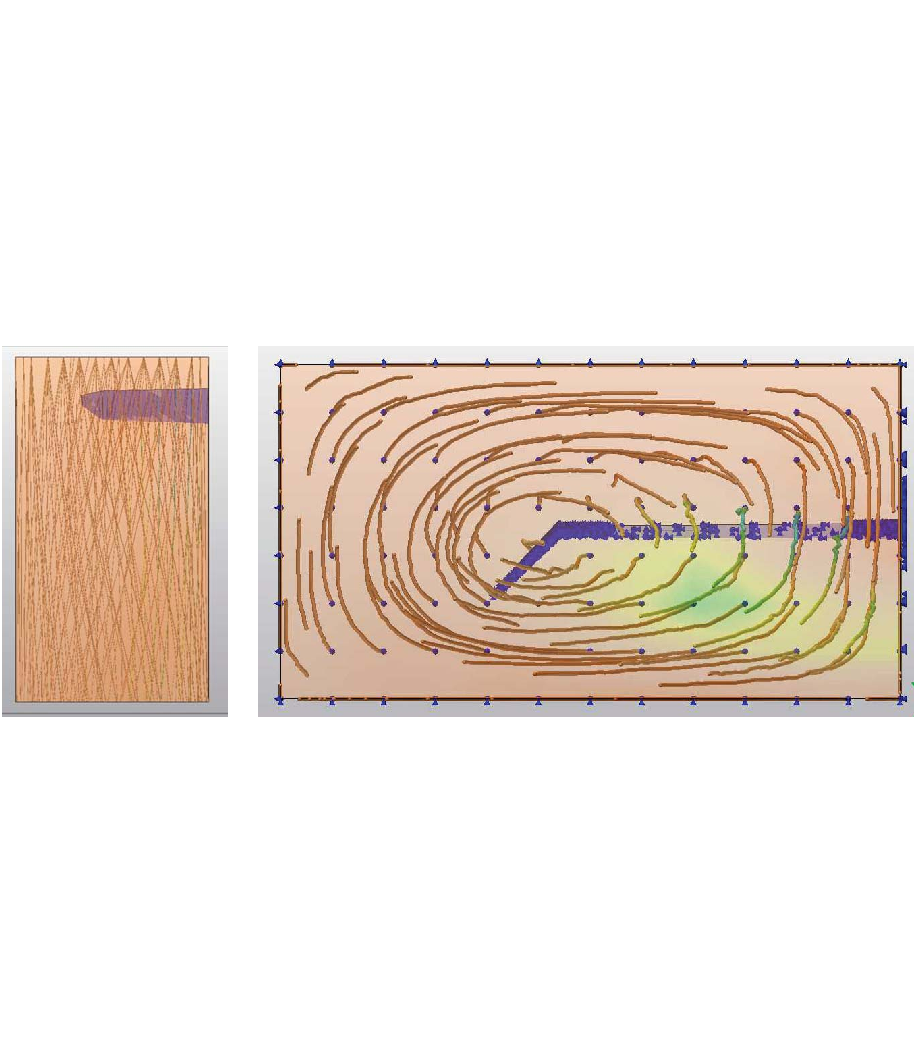
\includegraphics[]{obrazky/simulace/simulace7p}
	\caption{Simulce wingletu s odklonem $65\,^{\circ}$. Je vidět velký vír s velkou úhlovou rychlostí.}
	\label{sim:7}
\end{figure}

\begin{figure}[H]
	\centering
	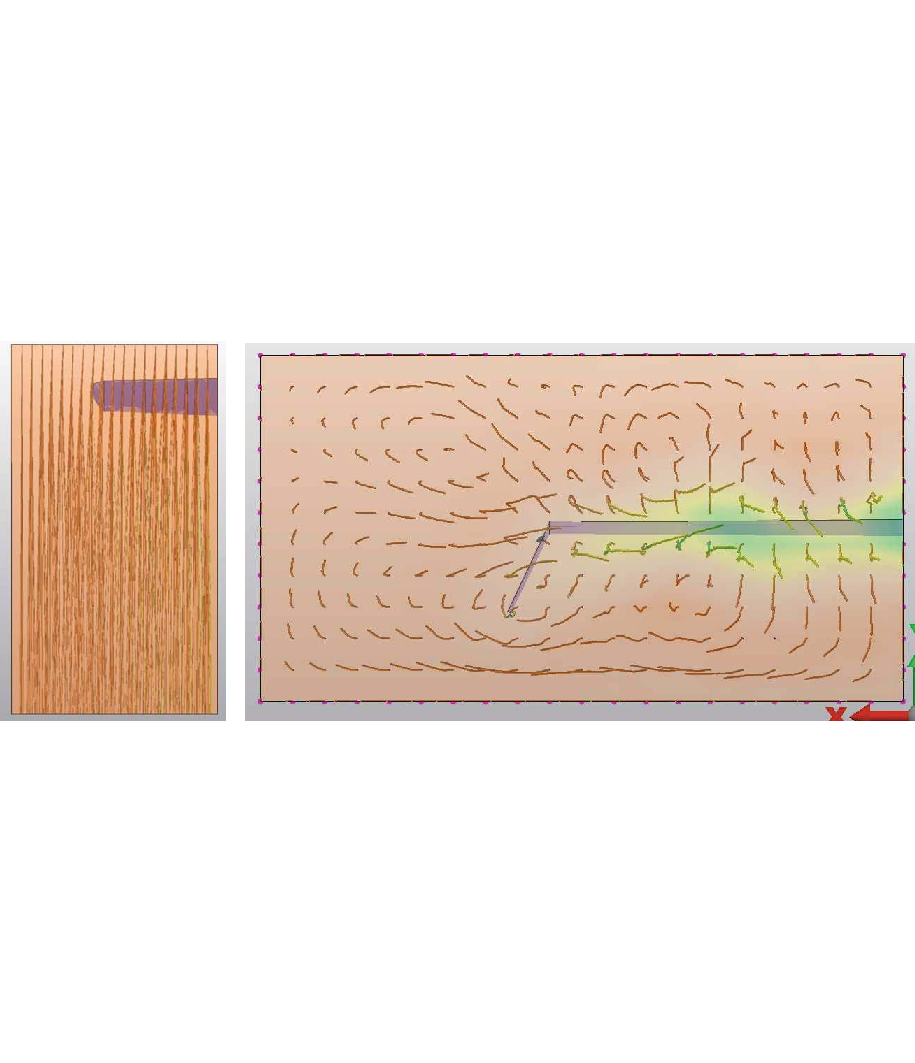
\includegraphics[]{obrazky/simulace/simulace8p}
	\caption{Simulace wingletu s odkolonem $85\,^{\circ}$. Tento wingletu vykazuje znatelně lepší výsledky než předchozí.}
	\label{sim:8}
\end{figure}
Tato simulace mě přesvědčila, že winglet je účinným řešením indukovaných ztrát, avšak také ukázala, jak choulostivá oblast zakončení listu je. I malá změna může výrazně omezit vznikající indukovaný vír, ale také jej může výrazně podpořit.

Ačkoliv jeden z mých modelů vykazoval dobré vlastnosti, rozhodl jsem se v tomto návrhu větrné turbíny winglety nepoužít. Jedná se o oblast s nejistými výsledky, které nemám nějak podložené. Avšak studium a experimenty s winglety neopouštím – rozhodně se nejedná o slepou uličku. Pouze je metoda pokusu a omylu značně neefektivní.

\subsection{Zakončení obloukem dozadu}

Na obrázku \ref{konec:3} se nachází zakončení listu obloukem dozadu. Jako inspiraci jsem si zde vzal zakončení křídel rychlostní RC modelů letadel. Toto zakončení se také často objevuje na koncích vrtulí letadel čí lodních šroubů určených pro velké rychlosti.

\begin{figure}[H]
	\centering
	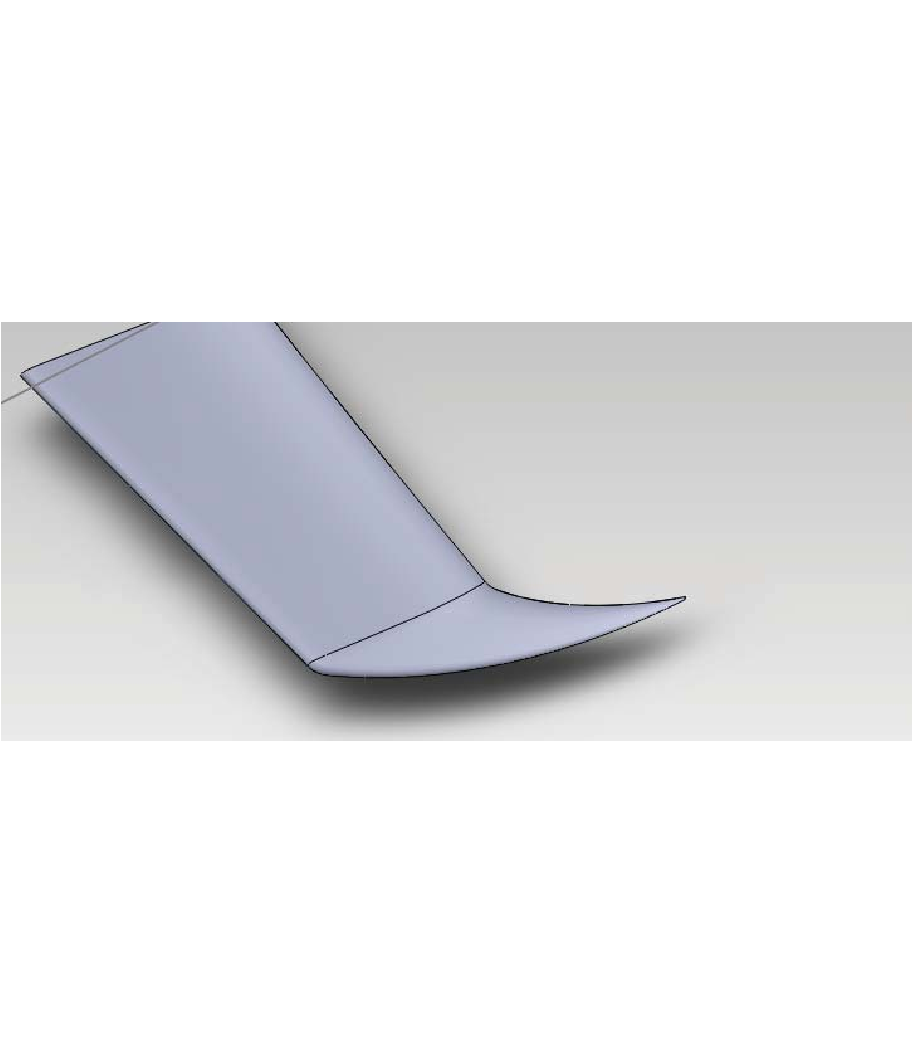
\includegraphics[]{obrazky/simulace/konec3p}
	\caption{Zakončení listu obloukem dozadu}
	\label{konec:3}
\end{figure}

Je důležité poznamenat, že tento oblouk je v rovině listu – není zahnutý. Bohužel však opět tento tvar nemám podložený teorií. I většina autorů výše uvedených modelů tvoří tato zakončení \uv{jen tak}.

Toto zakončení vytváří velký, ale relativně pomalý vír (obrázek \ref{sim:9}). Tento vír má podobné vlastnosti jako vír v případě odsazení. Na výsledcích simulace je vidět zrychlení víru, které je ovšem opět způsobeno působením stěn simulačního prostoru.

\begin{figure}[H]
	\centering
	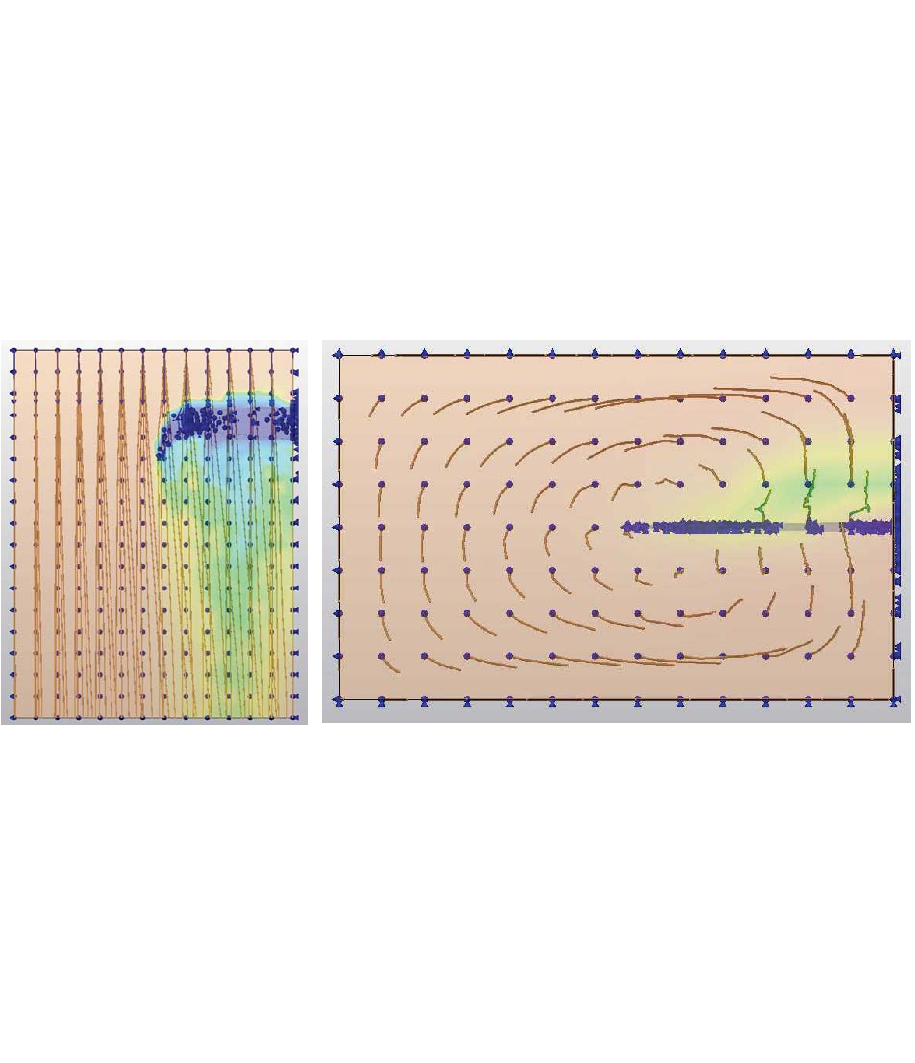
\includegraphics[]{obrazky/simulace/simulace9p}
	\caption{Výsledky simulace zakončení obloukem dozadu}
	\label{sim:9}
\end{figure}

\subsection{Zakončení kopulí}
Na spoustě malých větrných elektráren lze vidět zakončení listu kopulí. Toto zakončení je často používáno i na křídlech letadel. Model zakončení kopulí je na obrázku \ref{konec:4}.

\begin{figure}[H]
	\centering
	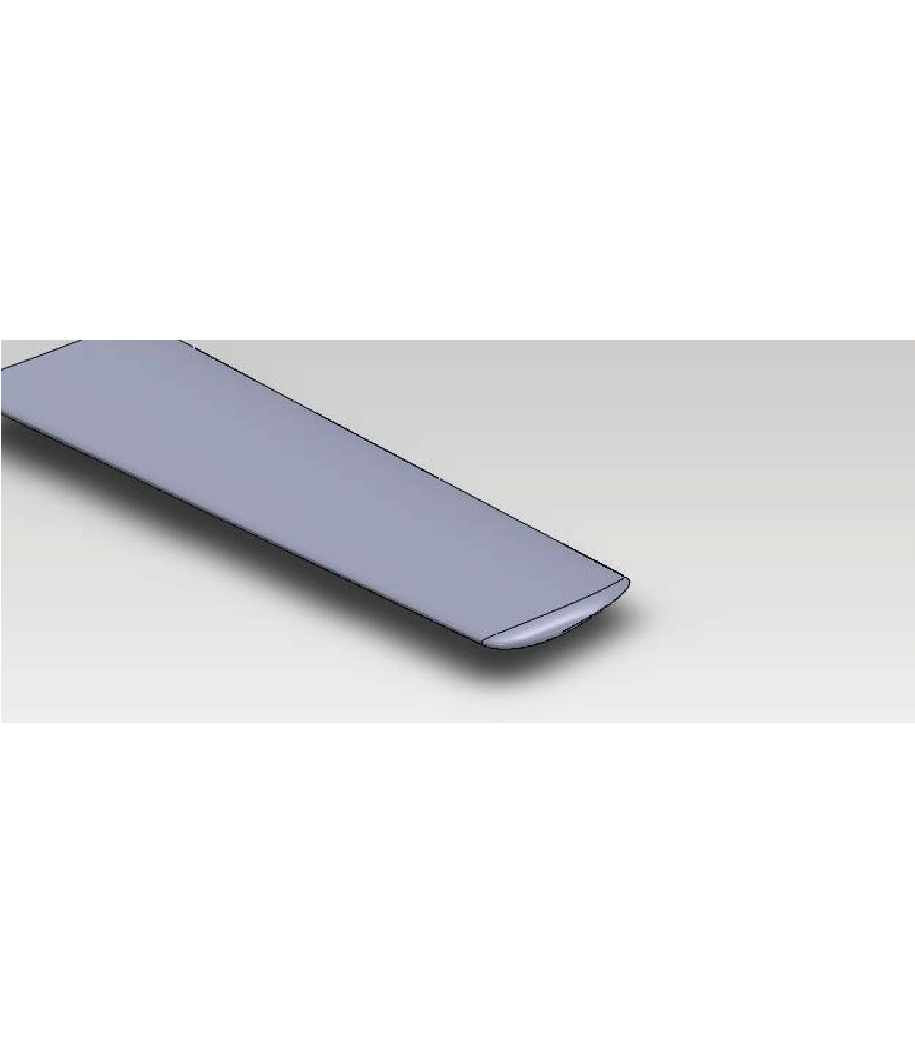
\includegraphics[]{obrazky/simulace/konec4p}
	\caption{Model zakončení listu obloukem}
	\label{konec:4}
\end{figure}

Od tohoto zakončení jsem očekával dobré výsledky – přece jen je hojně používané. Výsledky mě překvapily (obrázek~\ref{sim:10}). Na konci křídla vzniká velký vír s velkou úhlovou rychlostí. Pozitivem je, že tento vír nevzniká za aktivní plochou listu, tudíž jej příliš neovlivňuje.

\begin{figure}[H]
	\centering
	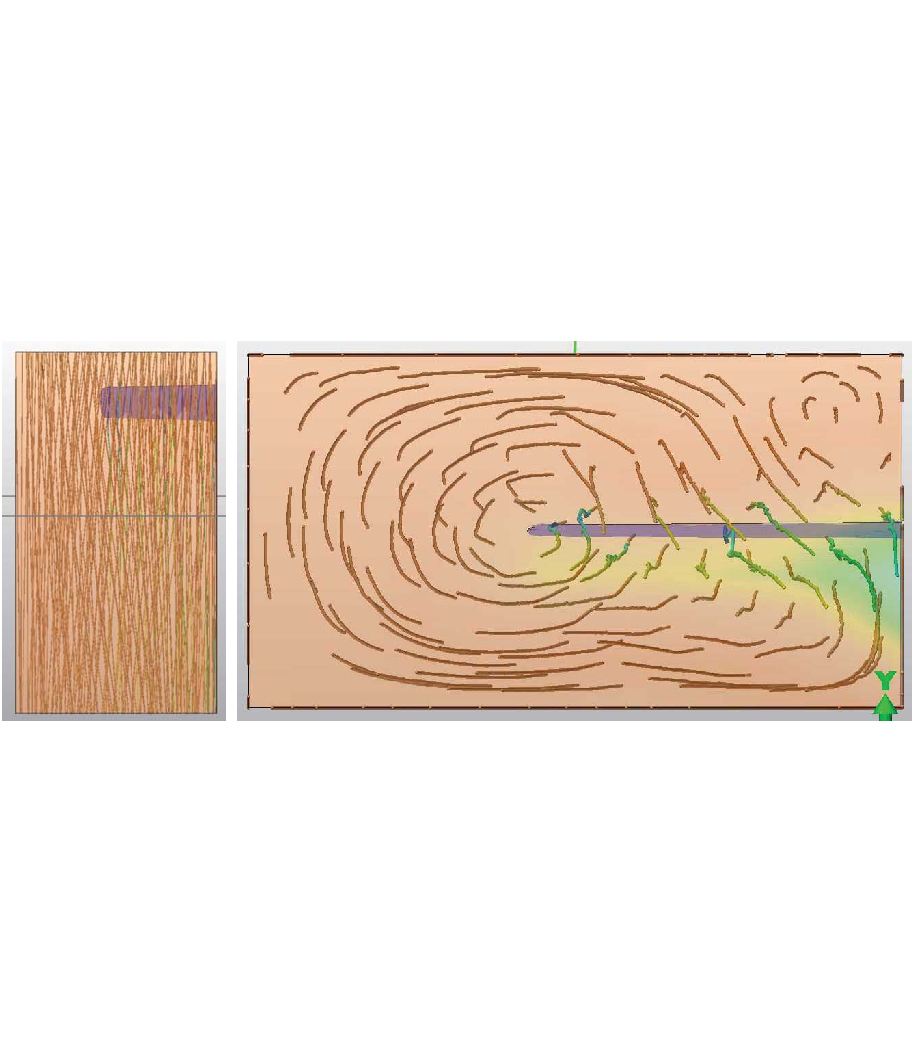
\includegraphics[]{obrazky/simulace/simulace10p}
	\caption{Výsledky simulace zakončení kopulí}
	\label{sim:10}
\end{figure}

Je však možné, že výhoda tohoto zakončení spočívá jinde. Díky tomu, že tečně navazuje na konec listu a jedná se o hladkou plochu bez ostrých hran, nevznikají na tomto zakončení chvění vzduchu způsobující hluk. Tuto domněnku však nemohu potvrdit – simulaci tohoto typu jsem nebyl schopen provést.

\subsection{Výběr zakončení}
Z výše uvedeného porovnání vyplývá, že dobré výsledky dává zakončení pětimilimetrovým odsazením, wingletem a obloukem dozadu.

Pro svůj model jsem použil odsazení, jelikož se jedná o tvar, ve kterém hraje roli jediná proměnná – velikost odsazení a ta jde jednoduše nasimulovat. Ostatní zakončení jsou komplexními tvary, které za některých okolností podávají dobré a za některých okolností špatné vlastnosti.
